\subsection{Analysis with Neural Network Model}

%%%%%%%%%%%%%%%%%%%%%%%%%%%%%%%%%%%%%%%%%%%%%%%%%%%%%%%%%%%%%%%%%%%%%
\subsubsection{Predicting Performance}
Using 49 firm characteristic feature variables listed in table \ref{table: Firm Characteristics by Category}, firstly, we fit the neural network model with the training dataset. Then, we carefully tune the model to get the optimal prediction in the validation dataset. The finalized hyperparameters and model settings are listed in Table \ref{table: model summary}. Then we use the fitted model to predict the next month stock returns in the testing dataset, and to make sure all the predictions are out of sample. We do the same thing by using different measures of stock returns for comparision and report the R-squared value in the testing dataset in Table \ref{table: full sample r2}. The first row of the table reports the R-squared value in the testing dataset by using 49 firm characteristic feature variables sololy. The model's performance does not exhibit significant variation across the different measures of stock returns, as the R-squared values in predicting different targets remain in the vicinity of 0.8\%. Among all the different measures of stock returns, CAPM abnormal return is predicted the most accurately by the model with 0.923\% R-squared value in the testing dataset, while FF3 abnormal returns predicted least accurately with R-squared value 0.763\% in the testing dataset.

As proved by large literatures such as \citet*{cochrane2005financial}, \citet*{welch2008comprehensive}, as well as what we have explored in section \ref{sec: univariate ls portfolios} before, there are some interaction effects between firm characteristic feature variables and macroeconomic conditions for predicting stock return. Hence, we add CFNAI index and investors sentiment data as describled in section \ref{sec: macro data} (since they can be potential indicators that can proxy macroeconomic conditions.) together with the 49 firm features for predicting. In table \ref{table: full sample r2}, the last 3 rows report the R-squared value by using firm characteristic data, CFNAI index data and investors sentiment data combined. Comparing the effectiveness of adding the CFNAI index and investor sentiment data in predicting stock returns, it is observed that the R-squared value increased significantly across various measures of stock returns, especially for adding investors' sentiment data. Furthermore, the model's performance improved the most when combining all feature variables (CFNAI data and investors' sentiment data together), irrespective of the measure of stock returns used. This suggests that both the CFNAI index and investor sentiment data are reliable proxies for capturing macroeconomic conditions when predicting stock returns, and must be considered when conducting such predictions.

Comparing the performance of the neural model across different measures of stock returns after adding CFNAI index and investor sentiment data revealed interesting findings. While the addition of these macroeconomic variables resulted in only a slight increase in the R-squared value in the testing dataset for predicting abnormal returns regardless of which factor models the abnormal returns derived from, however, it has a much greater impact on predicting stock excess returns, as reflected in the substantial increase in the R-squared value in the testing dataset from 0.811\% with only firm characteristic features to 4.005\% with firm characteristic features and all the macroeconomic condition indicators. Therefore, it can be inferred that macroeconomic data is highly beneficial for predicting excess returns, but its significance is not as pronounced when predicting abnormal returns. 

\begin{table}[!ht]
  \centering
  \caption{\textbf{Full Sample R-squared Value in Testing Dataset}}
  \label{table: full sample r2}
  \begin{tabular}{lcccc}
  \hline
  Features & CAPM & FF3 & FF5 & Excess \\ \hline
  Firm & 0.923 & 0.763 & 0.773 & 0.811 \\ 
  Firm + CFNAI & 0.966 & 0.816 & 0.821 & 1.458 \\ 
  Firm + SENT & 1.263 & 0.938 & 0.978 & 2.651 \\ 
  Firm + CFNAI + SENT & 1.396 & 1.011 & 0.998 & 4.005 \\ \hline
  \end{tabular}
  \begin{tablenotes}
    \footnotesize
    \item This table reports R-squared value for predicting stock abnormal reutrn and excess return in the testing dataset, with macroeconomic variables CFNAI index and investor sentiment index.
  \end{tablenotes}
\end{table}

%%%%%%%%%%%%%%%%%%%%%%%%%%%%%%%%%%%%%%%%%%%%%%%%%%%%%%%%%%%%%%%%%%%%%
\subsubsection{Neural Network Portfolios}

Next we build value weighted portfolios based on model's predictions. Each month we sort the stocks into deciles based on their predicted returns, in each decile we assign weights to each component stocks based on their market capitalization. It is important to note that this portfolio formulation process involves rebalancing the portfolios every month and does not consider transaction costs. Figure \ref{fig: portfolios cum return firm features} illustrates the portfolios' cumulative returns (We plot stock abnormal return derived from CAPM, FF3, FF5 models, and stock excess returns all together.) throughout the whole sample period, using only firm characteristic variables for the prediction\footnote{The results of the rest with different conbinations of predictors are listed in the Appendix \ref{sec:appendixb2}.}. The prediction based portfolios can be differentiated from good to bad regardless of which kind of measures used for sotck returns, by following this investing stratagy, we could achieve around 7 times cumulative abnormal returns across the sample period while avoiding potential losses at the same level. The portfolio spectrum is almost symmetrically allocated on both sides of the zero line for stock abnormal returns. In the panel (d) of this figure depicts the cumulative value weighted portfolios based on prediction for stock excess return. Different from abnormal returns, most of the portfolios present upward slops across time instead of nearly symmetrically distributed on the both sides on zero line. And the model can still differentiate between good and bad returns, investing in the top decile can achieve nearly 12 times excess return while investing in the bottom decile would result in a negative return across the whole sample period.

\begin{figure}[H]
  \centering
  \caption{\textbf{Cumulative Return of Portfolios Based on Prediction with Only Firm Features}}
  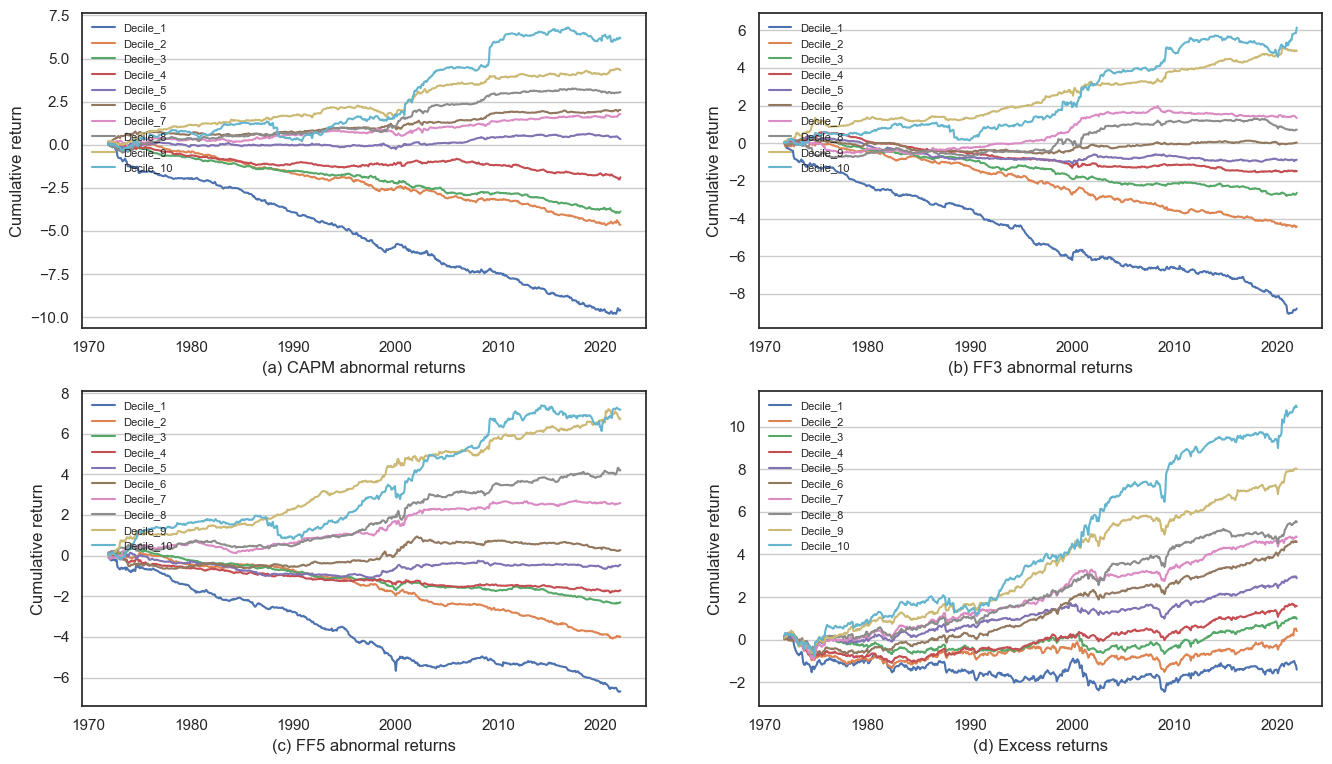
\includegraphics[width=.8\textwidth]{images/vw_portfolios_cumulative_return_firm.png}
  \label{fig: portfolios cum return firm features}
  \caption*{\footnotesize{This graphic shows the cumulative return of value weighted portfolios based on predictions with only firm characteristic feature variables.}}
\end{figure}

We employ the same strategy to formulate value-weighted portfolios based on predictions adding all macroeconomic variables, and explore the cumulative returns as depicted in Figure \ref{fig: portfolios cum return all features}. As we have explored before, the R-squared value in the testing dataset listed in Table \ref{table: full sample r2} is the highest when predicting with firm characteristic features and all macroeconomic variables together, which also indicating the greatest predicitng accuracy. The comparision between cumulative returns of value-weighted portfolios based on all variables and portfolios based solely on firm features supports the findings we have stated before. The top decile in each of the various measures of stock returns exhibits greater differentiation from the other deciles. Furthermore, there are slight improvements in distinguishing between the performance of other portfolios.

\begin{figure}[H]
  \centering
  \caption{\textbf{Cumulative Return of Portfolios Based on Prediction with All Features}}
  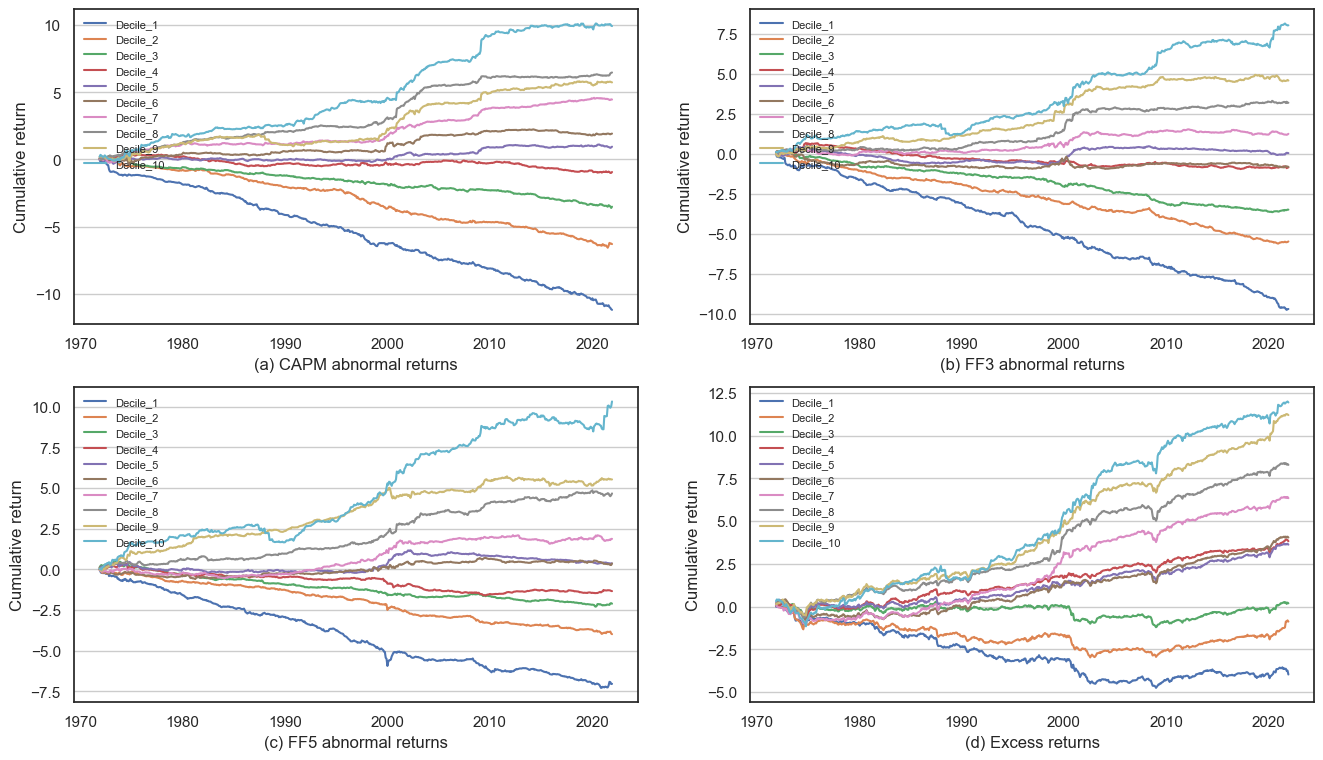
\includegraphics[width=.8\textwidth]{images/vw_portfolios_cumulative_return_all.png}
  \label{fig: portfolios cum return all features}
  \caption*{\footnotesize{This graphic shows the cumulative return of value weighted portfolios based on predictions with only firm characteristic and macroeconomic feature variables.}}
\end{figure}

%%%%%%%%%%%%%%%%%%%%%%%%%%%%%%%%%%%%%%%%%%%%%%%%%%%%%%%%%%%%%%%%%%%%
\subsubsection{Long-short Portfolios Based on Prediction}

In order to compare the performance of long-short portfolios based on model prediction with those based on univariate analysis, we first sort model predicted returns into deciles, then we select the top decile to long and the bottom decile to short, thereby constructing equally-weighted long-short portfolios. We plot the long-short portfolios' cumulative returns for various measures with different information sets in Figure \ref{fig: ls portfolios based on prediction}. The cumulative abnormal returns can exceed more than 25 times for portfolios formulated on prediction with both firm features and macroeconomic data. It is worth noting that in Figure \ref{fig: ff5 univariate ls cumulative return}, the best performance of univariate long-short portfolio based on short-term reversal only has achieved 20 times abnormal returns, and the majority of other univariate long-short portfolios did not generate cumulative abnormal returns of more than 10 times. When examining each panel in Figure \ref{fig: ls portfolios based on prediction}, we observe that the red line, representing the prediction-based long-short portfolios with both firm features and all macroeconomic data, dominates most of the other portfolios based on predictions with firm features alone or with a lack of CFNAI or sentiment data.

\begin{figure}[H]
  \centering
  \caption{\textbf{Cumulative Return of Long-short Portfolios Based on Prediction}}
  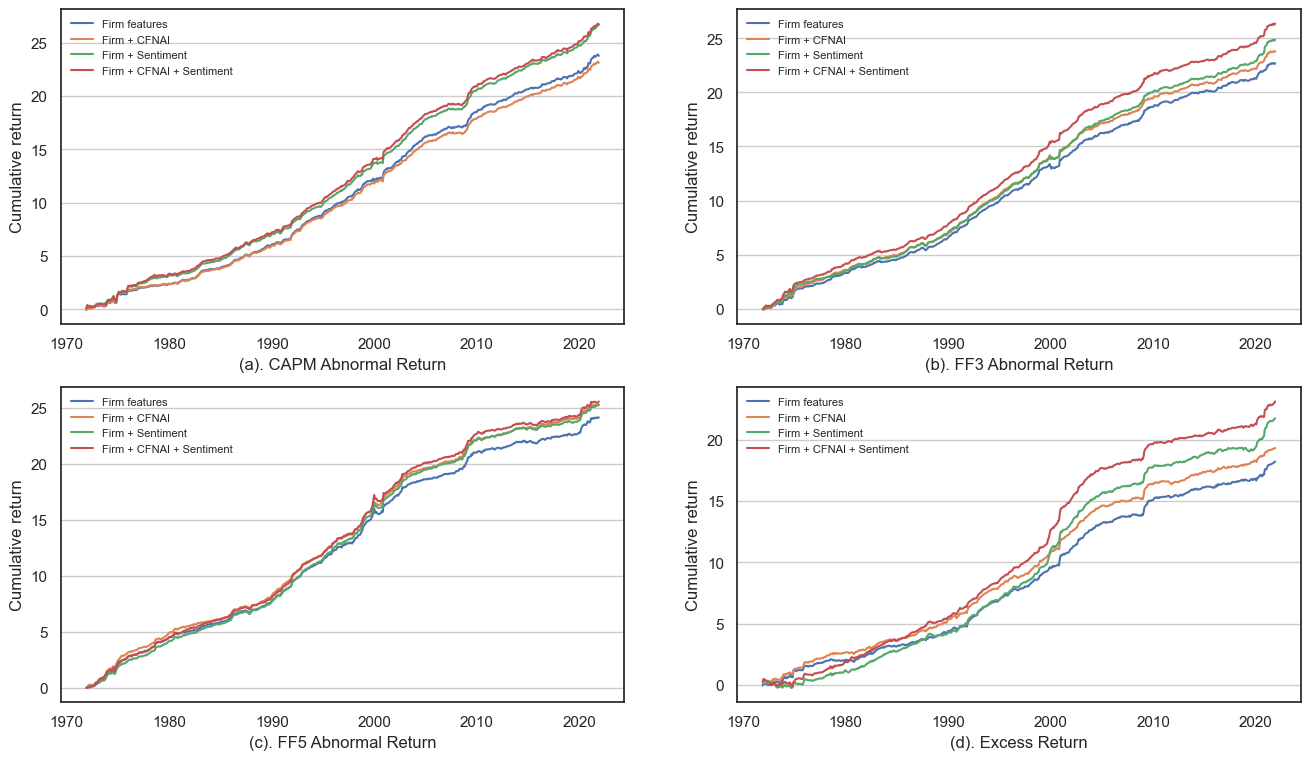
\includegraphics[width=.8\textwidth]{images/ls_portfolios_predictions.png}
  \label{fig: ls portfolios based on prediction}
  \caption*{\footnotesize{This graphic shows the cumulative return of long-short equal weighted portfolios based on predictions with only different conbinations of predictors.}}
\end{figure}
%%%%%%%%%%%%%%%%%%%%%%%%%%%%%%%%%%%%%%%%%%%%%%%%%%%%%%%%%%%%%%%%%%%%
\subsubsection{Feature Importance}

Next, we explore the relative importance of individual firm specific characteristics contributing to the final predicted outputs, as we have discussed in section \ref{subsec:feature importance} and also describled by \citet*{lundberg2018explainable}. Here we take the 3rd observation in the testing dataset as an example, as presented in figure \ref{fig: feature force 1st}, the actual output value of this observation is between (0, 0.02), and the model predicted return based on all the firm characteristics of this single observation is -0.06. The length of the force bar indicating how much a firm feature contributes to the predicted value, and the color represents whether a specific firm feature pushes the predicted output above or below the actual output value. In this case, the stock's Long Term Reversal (LRreversal) contributes the most to the predicted output, and followd by stock's Short Term Reversal (STreversal) and Beta. And features like Intermediate Momentum (IntMon), Momentum 12 Month (Mon12m), and Beta, etc,. push the predicted value above the actual output value. While, features like Long Term Reversal (LRreversal), Short Term Reversal (STreversal), Momentum Based on FF3 Residual (ResidualMomentum), etc,. push the predicted value below the actual output.

\begin{figure}[H]
  \centering
  \caption{\textbf{SHAP Feature Force No.1}}
  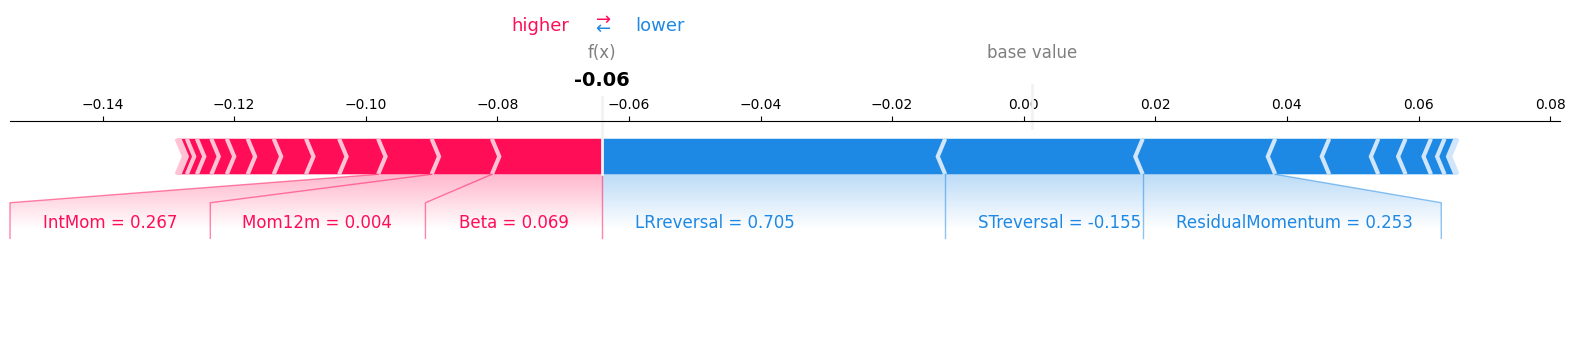
\includegraphics[width=.8\textwidth]{images/3rd_shap_feature_force.png}
  \caption*{\footnotesize{This graphic visulizes how each specific firm features contribute to the final predicted output. The numerical digits behind each features are the actual input values after scaling rounded to 3 decimals. The range is not necessarily between (-1,1), since we build the scaler based on the train data to scale all the train, validation and testing datasets.}}
  \label{fig: feature force 1st}
\end{figure}

Worth to mention that this one observation example does not represent the overall trending in the whole test sample. As you can see in figure \ref{fig: feature force 2nd} the contribution order of firm characteristics has changed for another observation. In this example, LRreversal and STreversal still contribute the most for predicting the output value of this observation, but instead of pushing the predicted stock return below the actual value, STreversal pushes the predicted stock return above the actural value in this example.

\begin{figure}[H]
  \centering
  \caption{\textbf{SHAP Feature Force No.2}}
  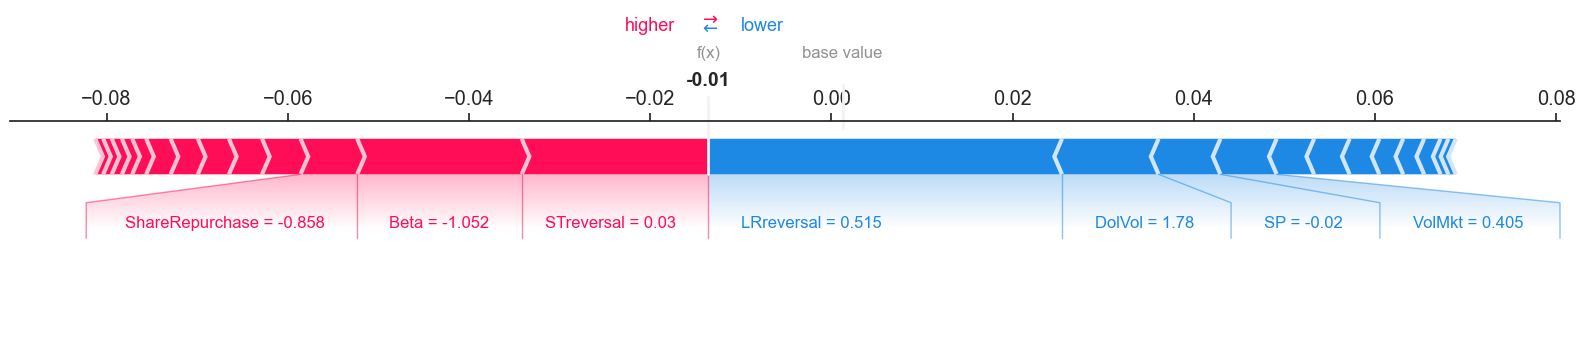
\includegraphics[width=.8\textwidth]{images/4th_shap_feature_force.png}
  \label{fig: feature force 2nd}
\end{figure}

Finally, we combine all the individual observations' Shap value to get the overall feature importance ranking as presented in Figure \ref{fig: feature importance ff5 ab}, for detailed explaination refering to \citet*{lundberg2017unified}. Panel (a) in the figure shows each firm variable's importance for predicting stock abnormal return, among which Short Term Reversla (STreversal) is the most important firm characteristic feature variable, followd by Past Trading Volumn (DolVol), 52 Weeks Trading High (High52) and Market Leverage (Leverage). In panel (b), we compute the mean Shap value within each group. The most important stock characteristic group is stock momentum, followd by trading fraction and macroeconomic variable investors sentiment, we have summarized the detailed group information in table \ref{table: Firm Characteristics by Category}.

\begin{figure}[H]
  \centering
  \caption{\textbf{Shap Feature Importance for FF5 Abnormal Return}}
  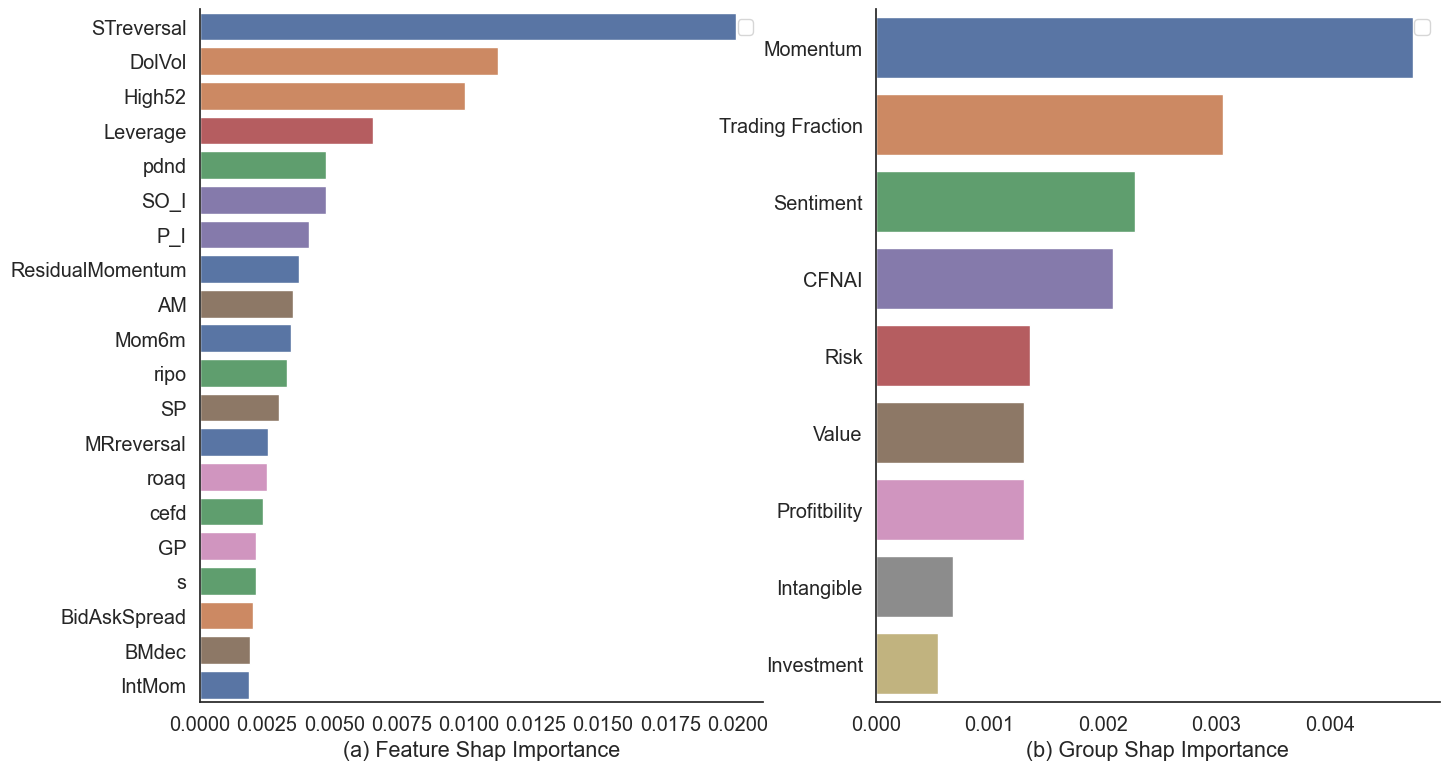
\includegraphics[width=.8\textwidth]{images/shap_feature_importance_ff5.png}
  \label{fig: feature importance ff5 ab}
  \caption*{\footnotesize{This figure shows the importance ranking for predictor variables and variable groups in predicitng stock abnormal returns derived FF5 factor model. The ranking is the average of the feature variables' Shap force. The variable importance measures are evaluated on the testing dataset. Group shap importance is the feature importance's sum value within each group.}}
\end{figure}

In the previous section, we declare that macroeconomic data is far more helpful in predicting stock excess return comparing to stock abnormal return based on the R-squared value. Figure \ref{fig: feature importance ex} dipicts Shap feature importance for stock excess return. Comparing it with figure \ref{fig: feature importance ff5 ab}, the ranking of variables importance has changed and macroeconomic variables ranked to the top above momentum, once again confirm that macroeconomic variables are extremly important for predicting stock excess return comparing to stock abnormal return. Remember equation \ref{eqn:abnormal return 1} and \ref{eqn:abnormal return 2}, stock abnormal return is defined as the alpha derived from factor model while stock excess return is just stock's log return in excess of risk free rate. The reason why stock abnormal return is not so relevant with macroeconomic data is probably because the factor model can capture some macroeconomic information, and it has been removed by the factor models\footnote{Feature importance for predicting stock abnormal returns derived from CAPM model and FF3 model are also presented in Appendix \ref{sec:appendixb3}.}.

\begin{figure}[H]
  \centering
  \caption{\textbf{Shap Feature Importance for Excess Return}}
  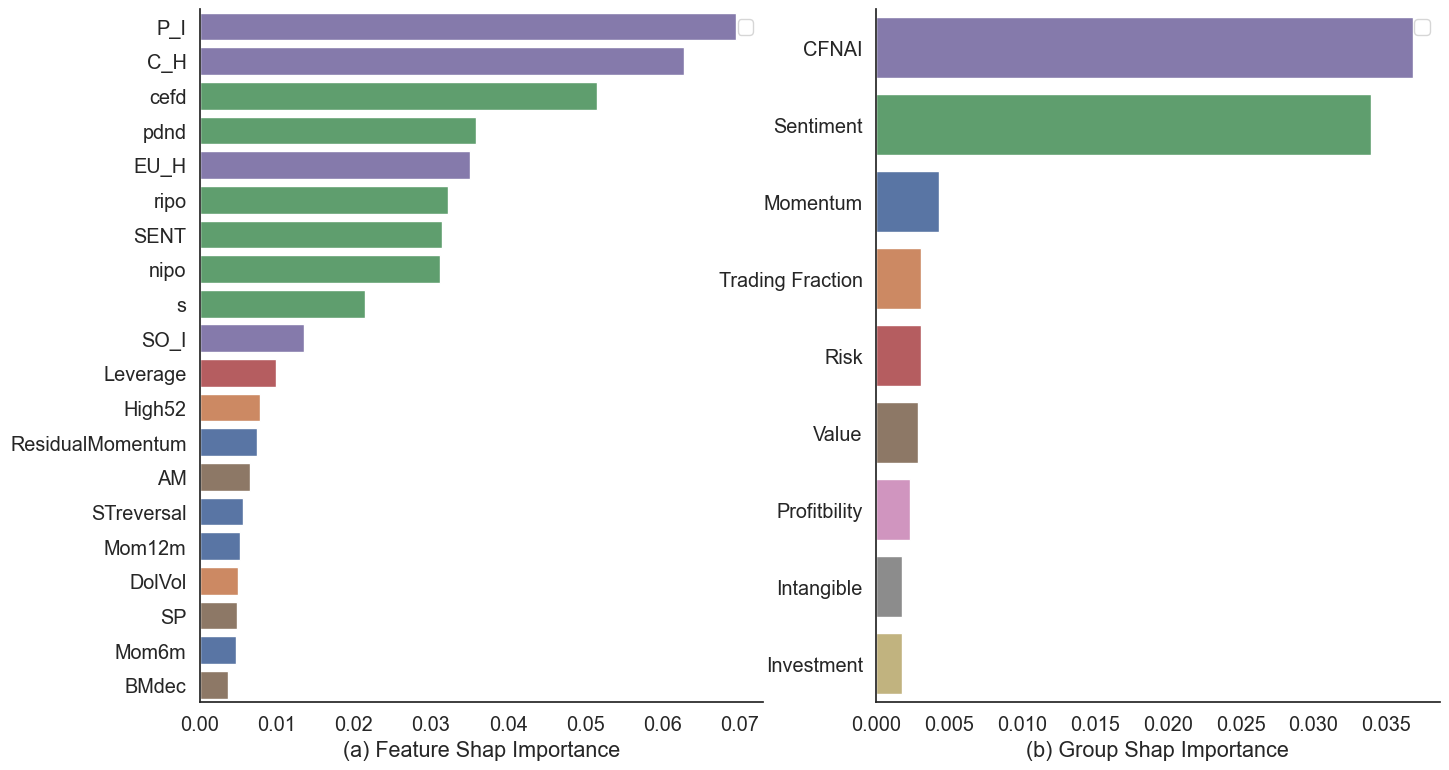
\includegraphics[width=.8\textwidth]{images/shap_feature_importance_ex.png}
  \label{fig: feature importance ex}
  \caption*{\footnotesize{This figure shows the importance ranking for predictor variables and variable groups in predicitng stock excess returns. The ranking is the average of the feature variables' Shap force. The variable importance measures are evaluated on the testing dataset. Group shap importance is the feature importance's sum value within each group.}}
\end{figure}
%%%%%%%%%%%%%%%%%%%%%%%%%%%%%%%%%%%%%%%%%%%%%%%%%%%%%%%%%%%%%%%%%%%

\subsubsection{Macroeconomic Variable Interaction Effects}

Neural network models have advantages accommodating potential complex interaction effects among predictors over other models. We have unveiled the tip of iceberg in section \ref{sec: univariate ls portfolios}, here we step deeper exploring the interaction effects between macroeconomic variable CFNAI index and firm characteristic features that are captured by neural network model. Figure \ref{fig: interaction effect_ex} plots a set of pairwise interaction effects captured by the neural network, it shows how expected stock return vary when we keep all other firm characteristic features fixed at their median value from the testing dataset simultaneously change one firm characteristic feature over the range (-1, 1) and different quantile values of CFNAI index. 

The upper left figure shows how the variable 52 Weeks Trading High (High52) affects predicted stock excess return, the non-linear relationship between this variable and stock excess return is captured by the neural network model, and the CFNAI index put different infuluence on the predicted stock return along with the change of this variable. It shows the macroeconomic condition (we consider CFNAI index proxies macroeconomic conditions) is more significant when the value of variable High52 is low. The interaction effects between variable High52 and CFNAI is clearly observed in this figure, worth to mention that if there is no interaction effects between these two variables the lines of different CFNAI level should be paralle. In panel (b), (c), (d), we also observe the similar interaction effects among CFNAI and momentum based on FF3 residuals (ResidualMomentum), medium‐run reversal (MRreversal), and short-term reversal (STreversal).

\begin{figure}[H]
  \centering
  \caption{\textbf{Interaction Effects Between Firm Features and CFNAI, Excess}}
  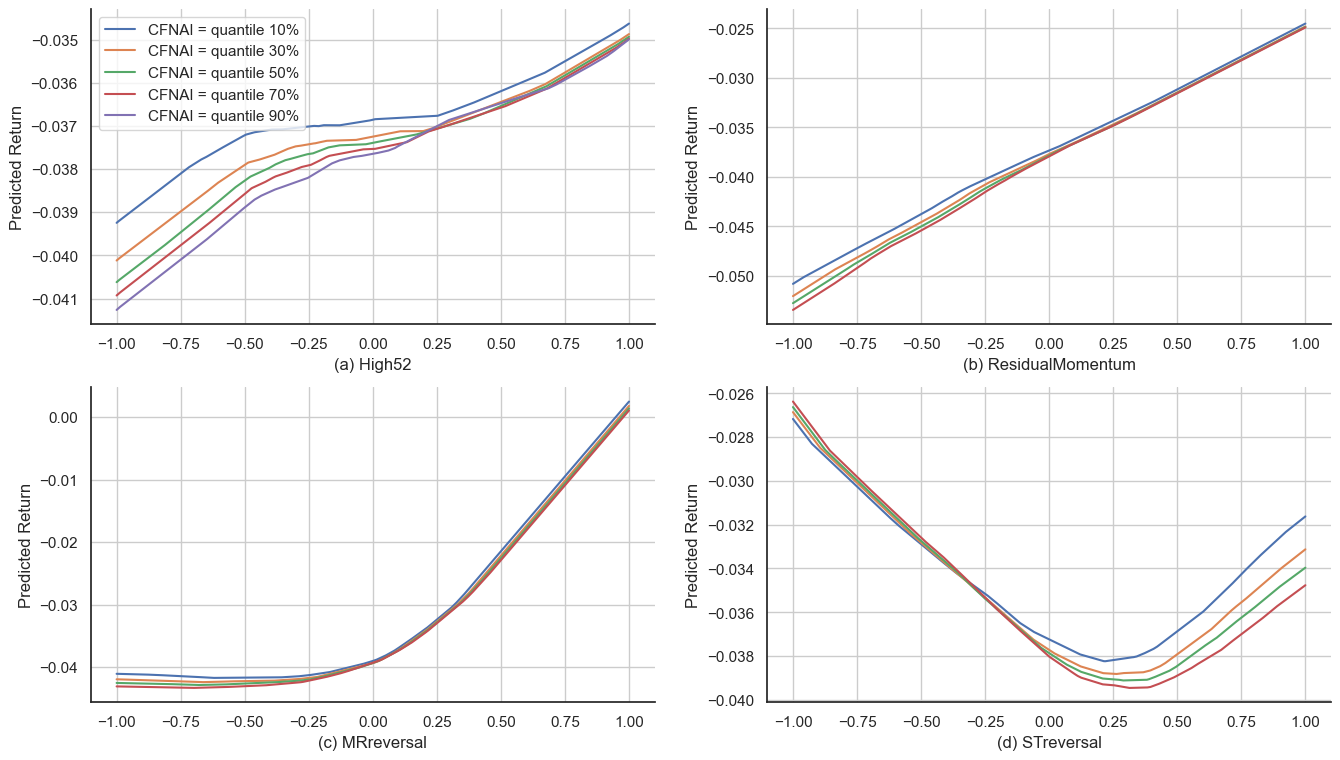
\includegraphics[width=.8\textwidth]{images/interactive_effect_excess.png}
  \label{fig: interaction effect_ex}
  \caption*{\footnotesize{This graphic shows the predicted stock excess return as a function of one stock characteristic feature variable, High52 (52 weeks trading high), ResidualMomentum (Momentum based on FF3 residuals  ), MRreversal (Medium‐run reversal), STreversal (Short term reversal) accordingly. The 'one' variable has a range between(-1, 1), macroeconomic variable CFNAI is seperated at 10\%, 30\%, 50\%, 70\%, and 90\% level. All other variables are fixed with the median value in the testing dataset.}}
\end{figure}

We also plot the interaction effects between the same variables and CFNAI index from the predicton of stock abnormal return derived from FF5 factors model in figure \ref{fig: interaction effect_ff5}. The interaction effect is not as strong as the predicton of stock excess return. In the figure, we could not observe clear interaction effects among these variables and CFNAI index. The reason behind again is that stock abnormal returns are not so relevant with macroeconomic conditions, which have been removed by factor models as we have discussed before.

\begin{figure}[H]
  \centering
  \caption{\textbf{Interaction Effects Between Firm Features and CFNAI, FF5}}
  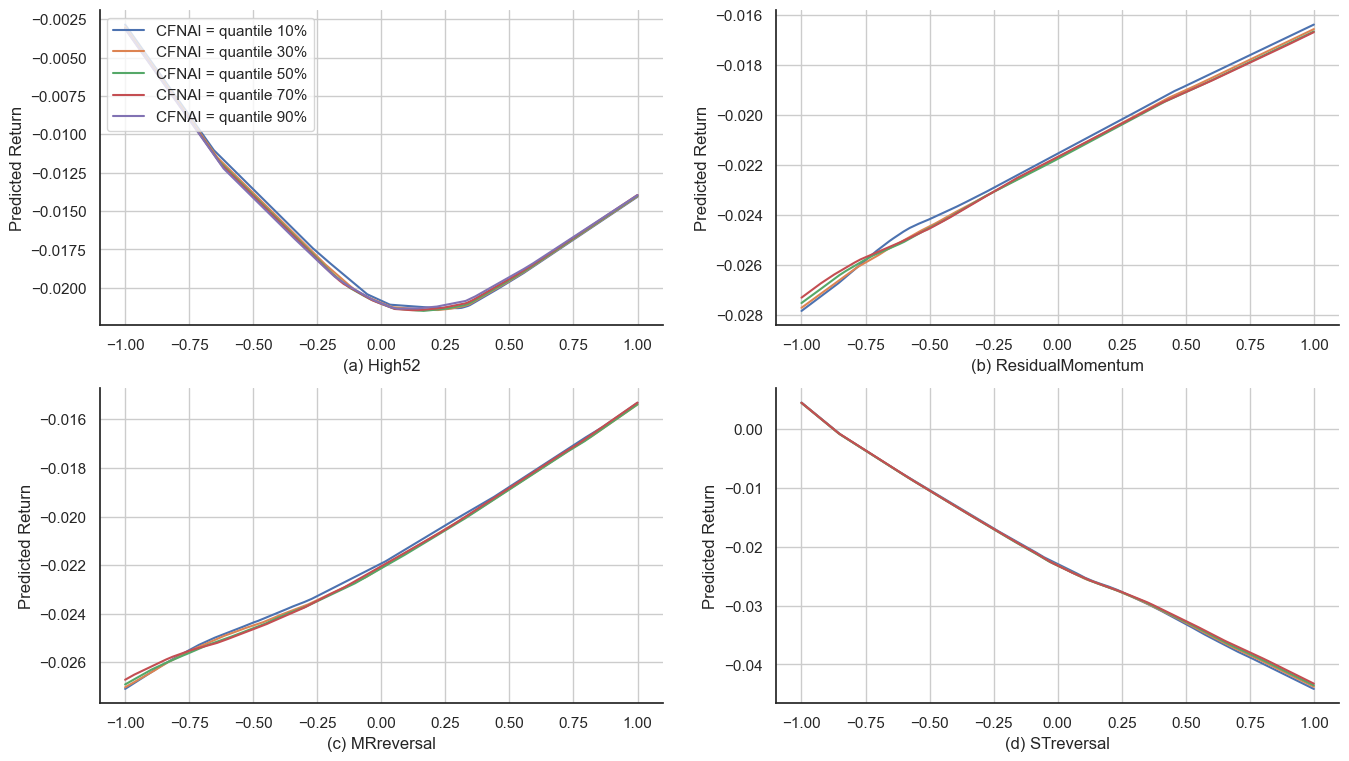
\includegraphics[width=.8\textwidth]{images/interactive_effect_ff5.png}
  \label{fig: interaction effect_ff5}
  \caption*{\footnotesize{This graphic shows the predicted stock abnormal return derived from FF5 factors model as a function of one stock characteristic feature variable, High52 (52 weeks trading high), ResidualMomentum (Momentum based on FF3 residuals  ), MRreversal (Medium‐run reversal), STreversal (Short term reversal) accordingly. The 'one' variable has a range between(-1, 1), macroeconomic variable CFNAI is seperated at 10\%, 30\%, 50\%, 70\%, and 90\% level. All other variables are fixed with the median value in the testing dataset.}}
\end{figure}

%%%%%%%%%%%%%%%%%%%%%%%%%%%%%%%%%%%%%%%%%%%%%%%%%%%%%%%%%%%%%%%%%%%
\subsubsection{Market Timing Based on Macroeconomic Conditions}

The interaction effects between macroeconomic conditions and firm feature variables have been shown to be strong, as demonstrated by the univariate long-short portfolios in Section \ref{sec: univariate ls portfolios} and the analysis above. Given this finding, the question arises as to whether the model prediction-based portfolios can achieve varying returns in different macroeconomic conditions, which would enable investors to identify optimal market timing for investment. Table \ref{table: portfolio ret in tertiles} shows the out-of-sample long-only portfolios' performance in different macroeconomic conditions. The portfolios are formulated based on the sorting of next-month model-predicted returns into deciles. We divide the CFNAI index into tertiles and define the bottom to top tertile as a recession, normal, and expansion period respectively. Within each period, the long-only portfolios achieve a clear increase in the mean portfolio's return for both stock abnormal and excess returns, which confirms that the model prediction-based portfolios are distinguished from bad to good. When considering Sharpe ratios instead of mean returns, the evidence is nearly identical, with higher deciles achieving higher Sharpe ratios than lower deciles in most cases. These results suggest that the model prediction-based portfolios may offer value to investors seeking to optimize their investment decisions by considering macroeconomic conditions.

Comparing the results horizontally in both Panel (a) and Panel (b), the top decile (portfolio decile\_10) achieves higher mean returns and Sharpe ratios in recession periods when the CFNAI index in low. This result coincides once again with the univariate long-short portfolios' performance discussed in Section \ref{sec: univariate ls portfolios}. The result simply indicating that investors who want to invest during recession period, when the market is more volatile, can earn higher abnormal and excess returns than with the same strategy during other periods, when the market is more stable. The same observations are presented in the Appendix \ref{sec:appendixb5} for stock abnormal returns derived from CAPM and FF3 factors models.

\begin{table}[H]
  \centering
  \caption{\textbf{Prediction Based Portfolios' Return in Defferent Macroeconomic Conditions}}
  \begin{tabular}{l|cc|cc|cc}
  \hline
      \multicolumn{7}{c}{(a) Portfolios' FF5 Abnormal Return (Mean)}\\\hline
      ~ & \multicolumn{2}{c}{Recession} & \multicolumn{2}{c}{Normal} & \multicolumn{2}{c}{Expansion} \\ \cline{2-7}
      Portfolios & Mean & Sharpe Ratio & Mean & Sharpe Ratio & Mean & Sharpe Ratio \\ \hline
      Decile\_1 & -1.779 & -0.367 & -1.823 & -0.443 & -1.564 & -0.347 \\ 
      Decile\_2 & -0.634 & -0.221 & -0.812 & -0.407 & -0.925 & -0.385 \\ 
      Decile\_3 & -0.716 & -0.292 & -0.348 & -0.234 & -0.533 & -0.221 \\ 
      Decile\_4 & -0.438 & -0.204 & -0.304 & -0.170 & -0.170 & -0.070 \\ 
      Decile\_5 & -0.179 & -0.070 & -0.148 & -0.088 & -0.135 & -0.054 \\ 
      Decile\_6 & 0.156 & 0.057 & 0.074 & 0.038 & -0.005 & -0.002 \\ 
      Decile\_7 & 0.220 & 0.074 & 0.323 & 0.161 & 0.031 & 0.015 \\ 
      Decile\_8 & 0.242 & 0.067 & 0.410 & 0.185 & 0.524 & 0.182 \\ 
      Decile\_9 & 1.199 & 0.256 & 0.923 & 0.300 & 0.958 & 0.288 \\ 
      Decile\_10 & 2.971 & 0.390 & 2.173 & 0.421 & 2.424 & 0.455 \\  \hline

      \multicolumn{7}{c}{(b) Portfolios' Excess Return (Mean)}\\\hline
      ~ & \multicolumn{2}{c}{Recession} & \multicolumn{2}{c}{Normal} & \multicolumn{2}{c}{Expansion} \\ \cline{2-7}
      Portfolios & Mean & Sharpe Ratio & Mean & Sharpe Ratio & Mean & Sharpe Ratio \\ \hline
      Decile\_1 & -0.345 & -0.048 & -0.450 & -0.072 & -0.380 & -0.052 \\ 
      Decile\_2 & 0.554 & 0.085 & 0.289 & 0.060 & -0.153 & -0.025 \\ 
      Decile\_3 & 0.461 & 0.075 & 0.485 & 0.110 & 0.138 & 0.025 \\ 
      Decile\_4 & 0.588 & 0.094 & 0.515 & 0.121 & 0.259 & 0.047 \\ 
      Decile\_5 & 0.703 & 0.108 & 0.661 & 0.144 & 0.305 & 0.051 \\ 
      Decile\_6 & 1.124 & 0.160 & 0.773 & 0.159 & 0.380 & 0.064 \\ 
      Decile\_7 & 1.263 & 0.175 & 0.957 & 0.196 & 0.373 & 0.061 \\ 
      Decile\_8 & 1.252 & 0.153 & 0.987 & 0.197 & 0.645 & 0.097 \\ 
      Decile\_9 & 2.094 & 0.241 & 1.303 & 0.244 & 0.978 & 0.138 \\ 
      Decile\_10 & 3.938 & 0.320 & 2.213 & 0.327 & 2.185 & 0.252 \\ \hline
  \end{tabular}
  \label{table: portfolio ret in tertiles}
  \begin{tablenotes}
    \footnotesize
    \item This table presents the actual mean portfolios' return and sharpe ratio in different macroeconomic conbinations. Portfolios are sorted based on the predicted abnormal and excess stock return made by neural network model. Macroeconomic conbinations defined as recession period, normal period, and expansion period based on the CFNAI index.
  \end{tablenotes}
\end{table}

%%%%%%%%%%%%%%%%%%%%%%%%%%%%%%%%%%%%%%%%%%%%%%%%%%%%%%%%%%%%%%%%%%%
